\documentclass{beamer}
\usetheme{CambridgeUS}
\usepackage[latin1]{inputenc}
\usefonttheme{professionalfonts}
\usepackage{times}
\usepackage{tikz}
\usepackage{amsmath}
\usepackage{verbatim}
\usetikzlibrary{arrows,shapes}
\usepackage[ruled,vlined]{algorithm2e}

\usepackage{listings}
\usepackage{xcolor}
\lstset{
    language=Python,
    basicstyle=\ttfamily\small,
    keywordstyle=\color{blue},
    commentstyle=\color{gray},
    stringstyle=\color{red},
    showstringspaces=false,
    breaklines=true,
    frame=single
}

\title{Comparing Model Architectures with k-Fold Cross-Validation}
\author{Fernando Pujaico Rivera}
\date{}

\begin{document}

\frame{\titlepage
\begin{tikzpicture}[remember picture, overlay]
\node[anchor=south east, xshift=0cm, yshift=1.0cm] 
at (current page.south east)
{
\includegraphics[width=2.5cm]{homepage.pdf}};
\end{tikzpicture}
}

%------------------------------------------------

\begin{frame}{A performs better than B?}
\begin{figure}
 \centering
 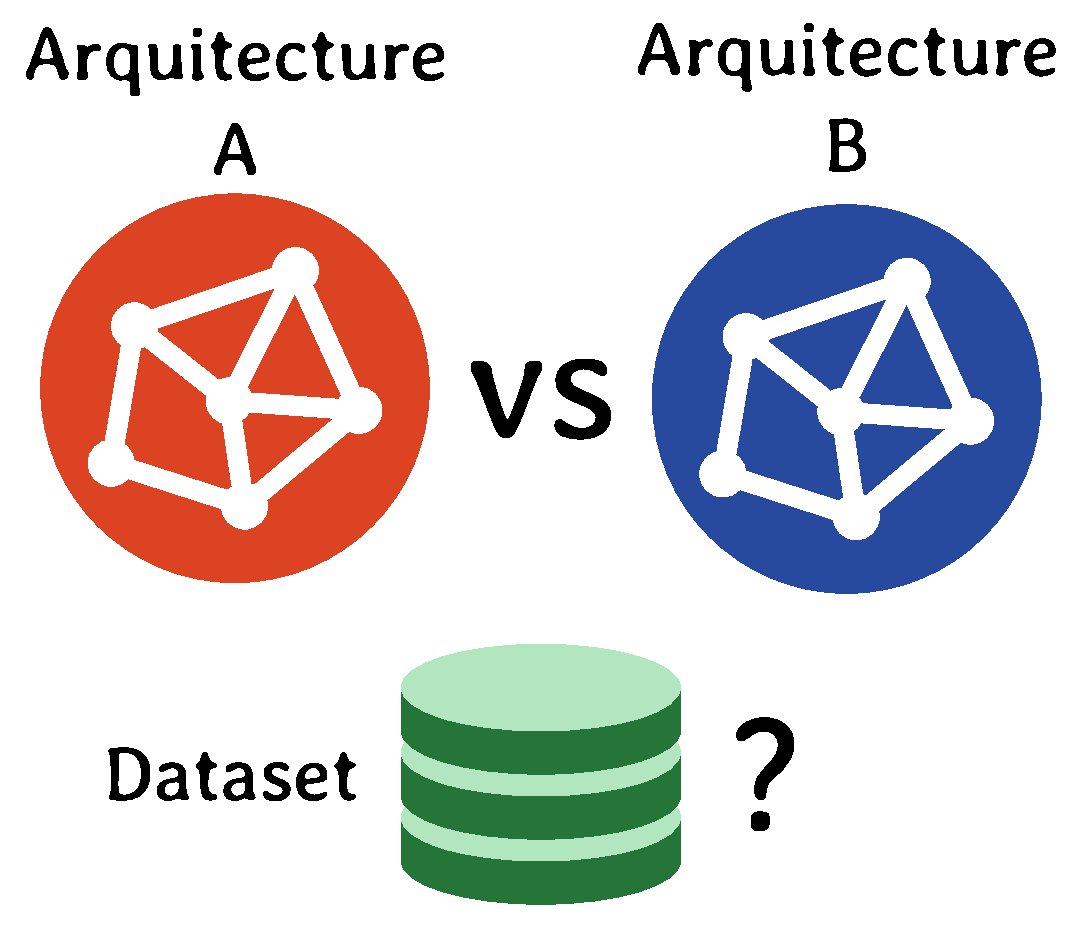
\includegraphics[width=0.65\linewidth]{dilema.pdf}
\end{figure}
\end{frame}

%------------------------------------------------

\begin{frame}{Problem}

\begin{description}
\item[Goal:] determine whether \textbf{Architecture A performs better than Architecture B}.
\bigskip
\item[Method:] \textbf{k-fold cross-validation} + \textbf{Wilcoxon signed-rank test}
\bigskip
\item[Objective:]
\begin{itemize}
\item Obtain multiple performance estimates
\item Perform a \textbf{statistical comparison between architectures}
\end{itemize}
\end{description}

\end{frame}

%------------------------------------------------

\begin{frame}{k-Fold Cross-Validation}
Dataset is divided into $K$ folds. If $K=5$, then

\begin{figure}
 \centering
 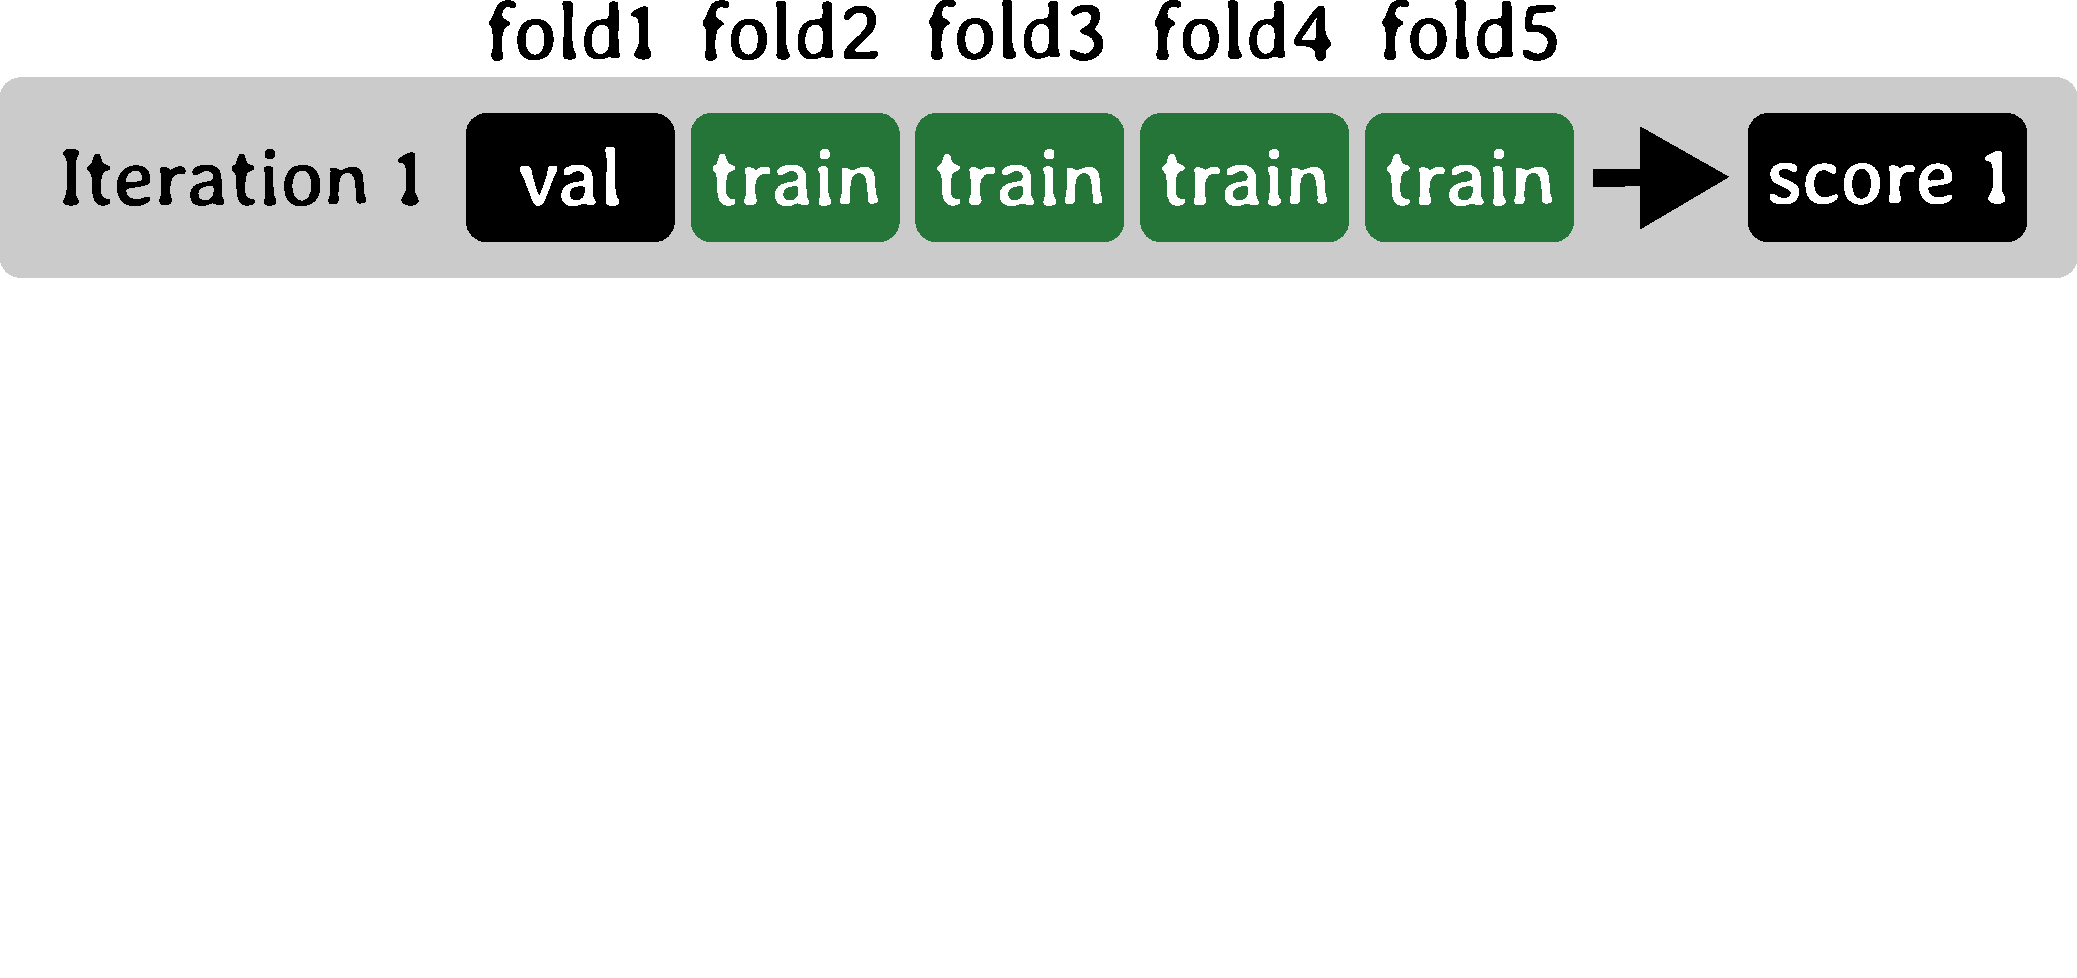
\includegraphics[width=0.95\linewidth]{kfold0.pdf}
\end{figure}

\end{frame}

\begin{frame}{k-Fold Cross-Validation}
Dataset is divided into $K$ folds. If $K=5$, then

\begin{figure}
 \centering
 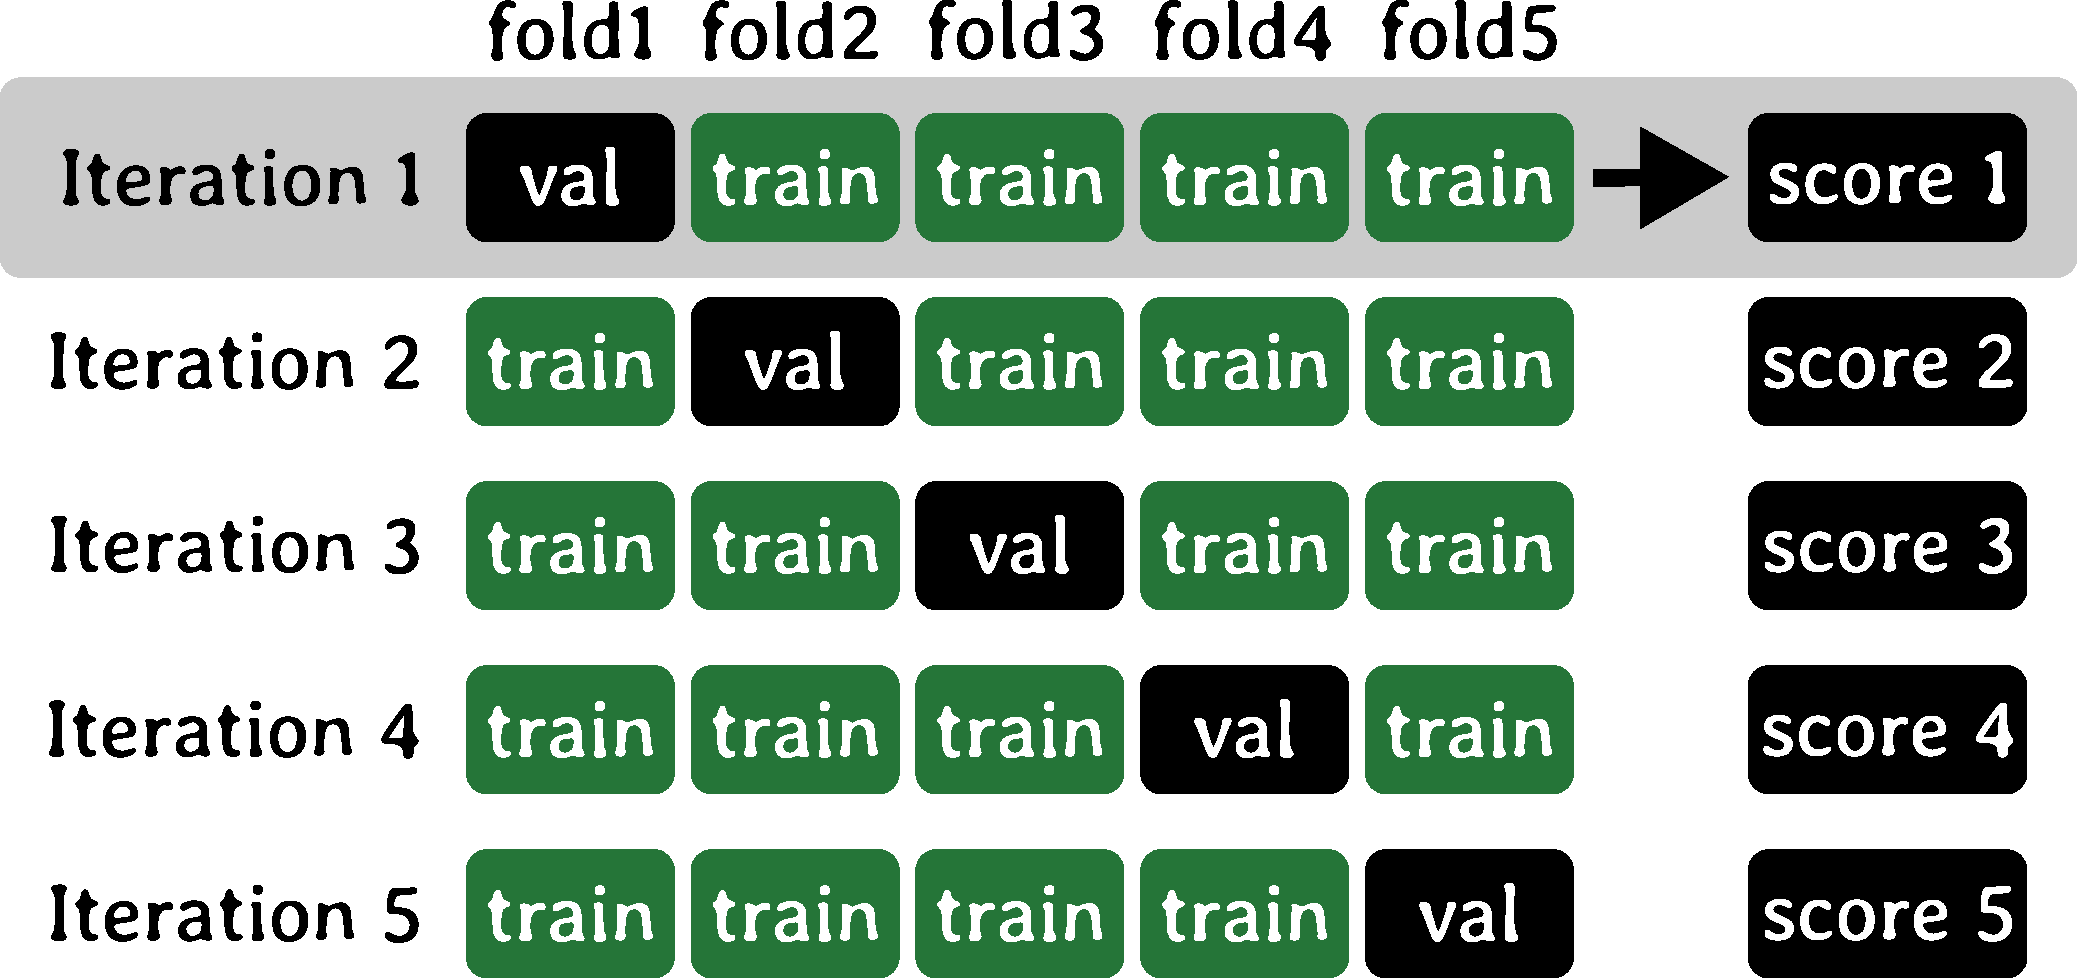
\includegraphics[width=0.95\linewidth]{kfold.pdf}
\end{figure}

\end{frame}

%------------------------------------------------

\begin{frame}{K-Fold Cross-Validation}
Example with $K = 5$.

\begin{center}
\begin{tabular}{c|c|c}
     & A & B \\
Validation fold & Score A & Score B \\
\hline
1 & $a_1$ & $b_1$ \\
2 & $a_2$ & $b_2$ \\
3 & $a_3$ & $b_3$ \\
4 & $a_4$ & $b_4$ \\
5 & $a_5$ & $b_5$
\end{tabular}
\end{center}

\[
\mu_A =\frac{1}{K}\sum_{k=1}^{K} a_{k}
\qquad
\mu_B =\frac{1}{K}\sum_{k=1}^{K} b_{k}
\]

\end{frame}

%------------------------------------------------

\begin{frame}{Paired Comparison}

Because both models are evaluated on the same folds, the comparison is \textbf{paired}.

\bigskip

For each fold:
\[
d_k = a_k - b_k
\]

\bigskip

We analyze the distribution of:
\[
\mathbf{d} = [d_1, d_2, d_3, d_4, d_5]
\]

\bigskip

\textbf{Key idea:}
We test whether the distribution of $d_k$ is centered above zero.
\end{frame}

%------------------------------------------------

\begin{frame}{Wilcoxon Signed-Rank Test}

\begin{center}
\Huge
\textcolor{blue}{Wilcoxon} \textcolor{red}{signed-rank test}
\end{center}

\bigskip

\textbf{What it tests:}
\begin{itemize}
\item Whether the distribution of paired differences $d_k = a_k - b_k$
\item is centered above zero
\end{itemize}

\bigskip

\textbf{Why not a t-test?}
\begin{itemize}
\item Does not assume normality
\item Works with small sample sizes
\item Based on ranks, not raw means
\end{itemize}

\end{frame}

%------------------------------------------------

\begin{frame}{Hypothesis Test}

We test whether model A tends to outperform model B.

\bigskip

Define:
\[
d_k = a_k - b_k
\]

\bigskip

\[
H_0 : \text{median}(\mathbf{d}) \le 0
\qquad
H_1 : \text{median}(\mathbf{d}) > 0
\]

\bigskip

\textbf{Interpretation:}
If $p < 0.05$, A tends to outperform B on the same folds.

\end{frame}

%------------------------------------------------

\begin{frame}[fragile]{Wilcoxon Test in Python}

\begin{tikzpicture}[remember picture, overlay]
\node[anchor=north east, xshift=0cm, yshift=-0.2cm] 
at (current page.north east)
{
\includegraphics[width=2.5cm]{qrcode.pdf}};
\end{tikzpicture}

\texttt{alternative="greater"} $\Rightarrow$ tests whether $d_k = A - B > 0$

\begin{lstlisting}
import numpy as np
from scipy import stats

A = np.array([0.82, 0.79, 0.83, 0.81, 0.80])
B = np.array([0.80, 0.76, 0.81, 0.78, 0.78])

stat, p = stats.wilcoxon(A, B, alternative="greater")

if p < 0.05:
    print("A performs significantly better than B")
\end{lstlisting}

\end{frame}

%------------------------------------------------

\begin{frame}{Important Limitation}

\textbf{Note:}

\begin{itemize}
\item Fold results are \textbf{not independent}
\item Training sets overlap across folds
\item Therefore, statistical tests on k-fold are \textbf{approximations}
\end{itemize}

\bigskip

\textbf{Implication:}
\begin{itemize}
\item Results should be interpreted with caution
\end{itemize}

\end{frame}

%------------------------------------------------

\begin{frame}{Conclusion}

Procedure:

\begin{enumerate}
\item Train models using \textbf{k-fold cross-validation}
\item Obtain paired scores $(a_k, b_k)$
\item Compute differences $d_k = a_k - b_k$
\item Apply a \textbf{one-sided Wilcoxon signed-rank test}
\end{enumerate}

\bigskip

\begin{algorithm}[H]
\eIf{$p < 0.05$}{
    We conclude that A tends to outperform B\;
}{
    No significant difference\;
}
\end{algorithm}

\end{frame}

%------------------------------------------------

\end{document}
